\def\beamerclassoptions{[xcolor=pdftex,dvipsnames,table,mathserif,aspectratio=169]}
% -----------------------------------------------------------------------------
% Thin wrapper preamble for Grad-IO slides
% Usage:
%  - Optionally set \def\beamerclassoptions{[<opts>]} before \input-ing this file
%    so a slide can control per-file beamer options (e.g. [handout,aspectratio=169]).
%  - This file ONLY issues the \documentclass once (honoring \beamerclassoptions)
%    and then loads the shared package `gradio-preamble.sty` which contains the
%    guarded package loads and macro definitions.
% -----------------------------------------------------------------------------
\ifdefined\beamerclassoptions
        % Expand \beamerclassoptions (which should be like "[notes=show]") safely
        \begingroup\edef\x{\endgroup\noexpand\documentclass\beamerclassoptions{beamer}}\x
\else
        \documentclass[handout,10pt,aspectratio=169]{beamer}
\fi

% Load the canonical shared preamble package. Try the local resources folder first
% so slide-level inputs continue to work in-place; if installed system-wide then
% \RequirePackage will also find it by name.
\IfFileExists{./gradio-preamble.sty}{\RequirePackage{./gradio-preamble}}{%
    \IfFileExists{gradio-preamble.sty}{\RequirePackage{gradio-preamble}}{%
        \RequirePackage{gradio-preamble}% final fallback to system-installed package
    }
}

% Any slide-specific packages or macros should be declared in the slide file
% after `% -----------------------------------------------------------------------------
% Thin wrapper preamble for Grad-IO slides
% Usage:
%  - Optionally set \def\beamerclassoptions{[<opts>]} before \input-ing this file
%    so a slide can control per-file beamer options (e.g. [handout,aspectratio=169]).
%  - This file ONLY issues the \documentclass once (honoring \beamerclassoptions)
%    and then loads the shared package `gradio-preamble.sty` which contains the
%    guarded package loads and macro definitions.
% -----------------------------------------------------------------------------
\ifdefined\beamerclassoptions
        % Expand \beamerclassoptions (which should be like "[notes=show]") safely
        \begingroup\edef\x{\endgroup\noexpand\documentclass\beamerclassoptions{beamer}}\x
\else
        \documentclass[handout,10pt,aspectratio=169]{beamer}
\fi

% Load the canonical shared preamble package. Try the local resources folder first
% so slide-level inputs continue to work in-place; if installed system-wide then
% \RequirePackage will also find it by name.
\IfFileExists{./gradio-preamble.sty}{\RequirePackage{./gradio-preamble}}{%
    \IfFileExists{gradio-preamble.sty}{\RequirePackage{gradio-preamble}}{%
        \RequirePackage{gradio-preamble}% final fallback to system-installed package
    }
}

% Any slide-specific packages or macros should be declared in the slide file
% after `% -----------------------------------------------------------------------------
% Thin wrapper preamble for Grad-IO slides
% Usage:
%  - Optionally set \def\beamerclassoptions{[<opts>]} before \input-ing this file
%    so a slide can control per-file beamer options (e.g. [handout,aspectratio=169]).
%  - This file ONLY issues the \documentclass once (honoring \beamerclassoptions)
%    and then loads the shared package `gradio-preamble.sty` which contains the
%    guarded package loads and macro definitions.
% -----------------------------------------------------------------------------
\ifdefined\beamerclassoptions
        % Expand \beamerclassoptions (which should be like "[notes=show]") safely
        \begingroup\edef\x{\endgroup\noexpand\documentclass\beamerclassoptions{beamer}}\x
\else
        \documentclass[handout,10pt,aspectratio=169]{beamer}
\fi

% Load the canonical shared preamble package. Try the local resources folder first
% so slide-level inputs continue to work in-place; if installed system-wide then
% \RequirePackage will also find it by name.
\IfFileExists{./gradio-preamble.sty}{\RequirePackage{./gradio-preamble}}{%
    \IfFileExists{gradio-preamble.sty}{\RequirePackage{gradio-preamble}}{%
        \RequirePackage{gradio-preamble}% final fallback to system-installed package
    }
}

% Any slide-specific packages or macros should be declared in the slide file
% after `\input{.../resources/preamble.tex}`.

`.

`.


\usetheme{metropolis}
%\usetheme{Darmstadt}
%\usepackage{times}
%\usefonttheme{structurebold}

\usepackage[english]{babel}
%\usepackage[table]{xcolor}
\usepackage{pgf,pgfarrows,pgfnodes,pgfautomata,pgfheaps}
\usepackage{amsmath,amssymb,setspace}
\usepackage[latin1]{inputenc}
\usepackage[T1]{fontenc}
\usepackage{relsize}
\usepackage[absolute,overlay]{textpos} 
\newenvironment{reference}[2]{% 
  \begin{textblock*}{\textwidth}(#1,#2) 
      \footnotesize\it\bgroup\color{red!50!black}}{\egroup\end{textblock*}} 

\DeclareMathSizes{10}{10}{6}{6} 


\title [Dynamic Oligopoly I]{Network Effects}
\author{C.Conlon }
\institute{Grad IO }
\date{Fall 2023}
\setbeamerfont{equation}{size=\tiny}
\begin{document}

\begin{frame}
\titlepage
\end{frame}

\begin{frame}{What are Network Effects?}
\begin{itemize}
\item An important aspect of many digital markets today is \textit{network effects}.
\item Main idea is that you value the good more if other people use it.
\begin{itemize}
\item Social Networks: Facebook, Instagram, Twitter, Tindr, etc.
\item Statistical Packages: Stata, R, Matlab, etc.
\item P2P Platforms: Ebay, Etsy, Alibaba, Uber.
\item Software Platforms: iOS, Android, Windows.
\item Game Consoles: PS4, XBox One, etc.
\end{itemize}
\item This creates a \alert{lock in} effect.
\begin{itemize}
\item You may have an incentive to underprice initially to drive adoption.
\item There may be benefits to being early to market.
\item Markets can \alert{tip} one way or another.
\end{itemize}
\item Two-sided markets are another important issue (Developers, Developers, Developers!) 
\end{itemize}
\end{frame}


\begin{frame}{What are Network Effects?}
\begin{itemize}
\item Consumers make adoption decision that is durable (or irreversible) and depends on two things:
\begin{itemize}
\item The share of users on the same platform $\rho_{jt}$
\item Beliefs about the future of $E[\rho_{j,t}]$
\end{itemize}
\item Because beliefs are important, multiple equilibria can arise
\item How do we measure the size/impact of indirect network effects?
\item Constructing a counterfactual equilibria in a world without network-effects is hard to do in practice.
\end{itemize}
\end{frame}

\begin{frame}{What are Network Effects?}
\begin{center}
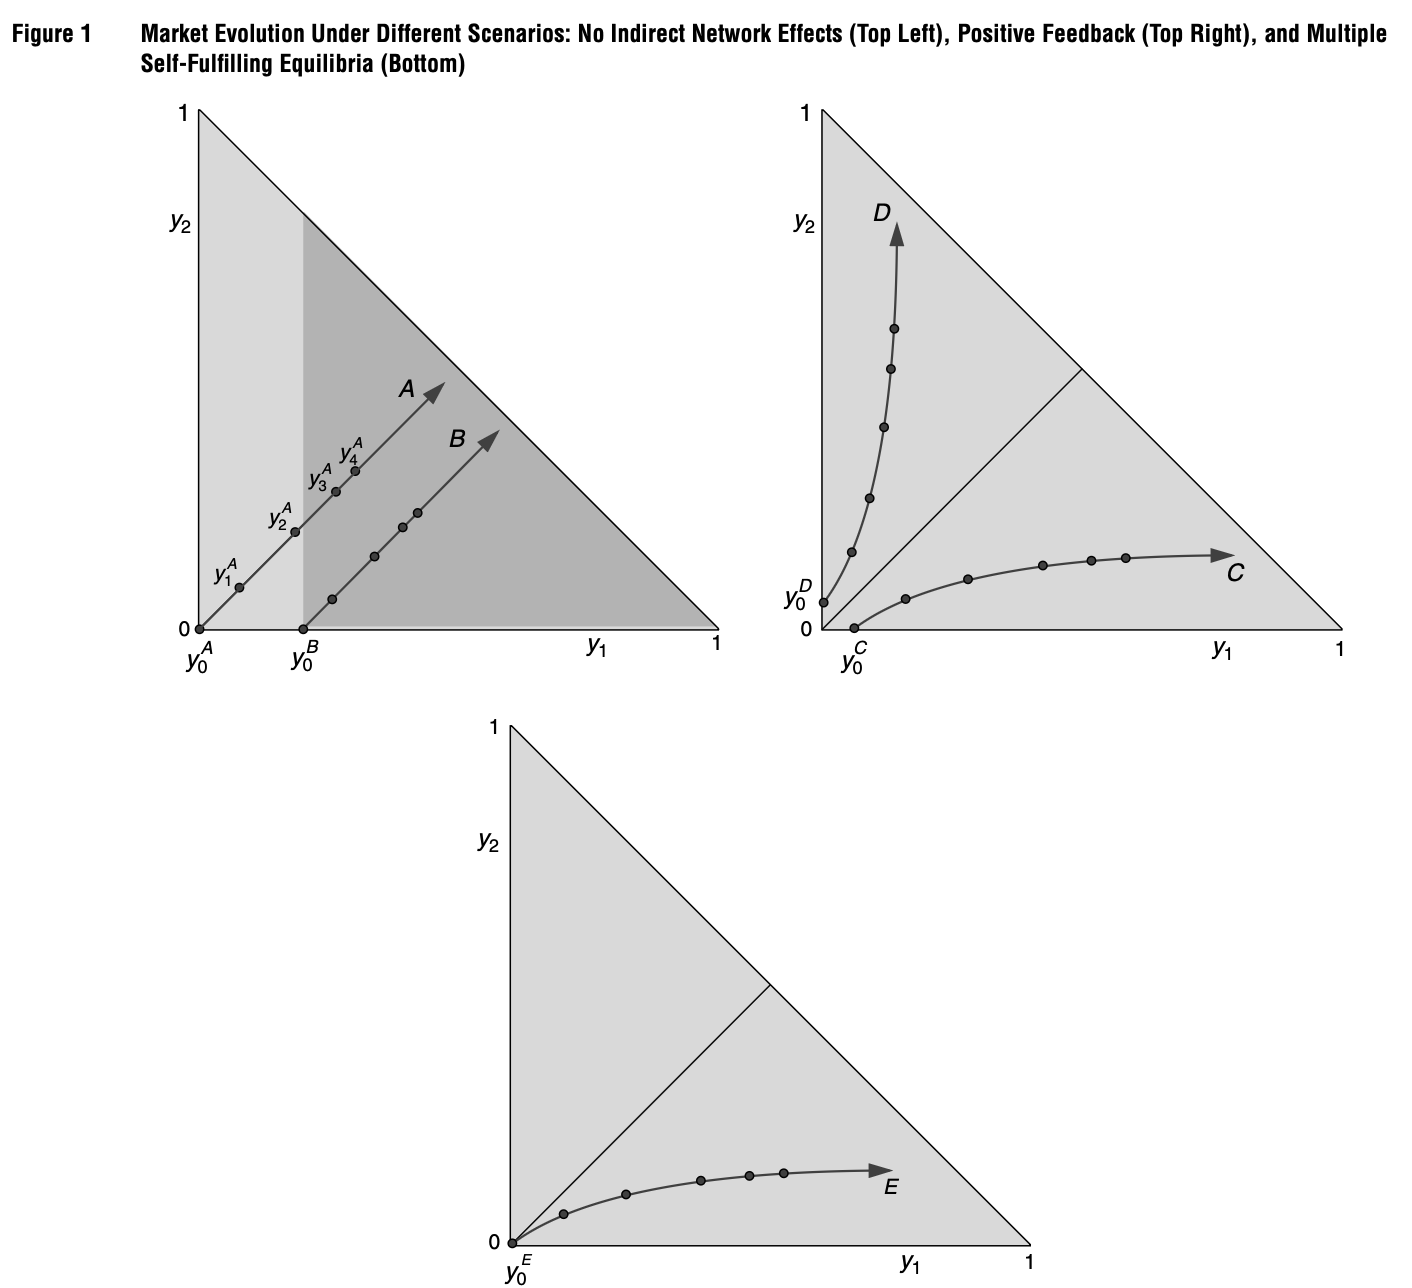
\includegraphics[scale=0.5]{resources/triangles.pdf}
\end{center}
\end{frame}


\begin{frame}{Dube, Hitsch, Chintagunta: Tipping}

\begin{itemize}
\item Start with two firms and $M=1$ mass of consumers
\item Installed base $y_{t} = [y_{1t},y_{2t}] \in [0,1]$ is the state space.
\item Assume that demand shock $\xi_{jt}~\sim \phi(\xi)$ is private information to the firm (similar to Seim's paper on video stores).
\item Timing of the game:
\begin{enumerate}
\item Firms learn $\xi_{jt}$ and set $p_{jt}$
\item Consumers adopt $\{1,2\}$ or delay purchase $=0$
\item Software firms supply a given number of titles $n_{jt}$
\item Sales are realized and firms receive profits. Consumers receive utility from $n_{jt}$ and in adoption period from platform itself.
\end{enumerate}
\item Information structure guarantees a unique best response (conjecture) and a pure-strategy equilibria.
\item Hence prices $p_{jt}$ contain a lot of information.
\end{itemize}
\end{frame}



\begin{frame}{}
\begin{itemize}
\item Titles depend on next period state variable: $n_{jt} = h_j(y_{j,t+1})$. Why?
\end{itemize}
\end{frame}

\begin{frame}{Consumers}
Need two things:
\begin{itemize}
\item Current prices and installed base $(p_t, y_t)$
\item Beliefs about the future $y_{t+1} = f^e(y_t,\xi_t)$ and conjecture about firm policy $p_{jt} = \sigma_j^e(y_t,\xi_t)$.
\end{itemize}
Utilities
\begin{itemize}
\item Flow from software: $u_j(y_{j,t+1}) = \gamma n_{jt} = \gamma h_j (y_{j,t+1})$
\item In PDV: $\omega_j (y_{t+1}) = E [ \sum_{k=0}^{\infty} \beta^k u_j(y_{j,t+1+k}) | y_{t+1}]$
\item This PDV trick is common (and helpful) and solves the recursion:
\begin{eqnarray*}
\omega_j(y_{t+1}) &=& u_j(y_{j,t+1}) + \beta \int  \omega_j( f^e(y_t,\xi_t)) \phi(\xi) \partial \xi\\
\end{eqnarray*}
\end{itemize}
\end{frame}

\begin{frame}{Consumers}
Choose $j$ to maximize choice specific value function (indirect utility) logit error :
\begin{eqnarray*}
v_j (y_t,\xi_t,p_t) &=& \delta_j + \omega_j( f^e(y_t,\xi_t)) - \alpha p_{jt} + \xi_{jt}\\
v_0(y_t,\xi_t) &=& \beta \int \max\{ v_0(y_{t+1},\xi) + \varepsilon_0, \\
&&  \max_j [v_j (y_{t+1},\xi_t,\sigma^e(y_{t+1},\xi)) + \varepsilon_j ] \} \cdot \phi(\xi) \phi_{\varepsilon}(\varepsilon)
\end{eqnarray*}
This gives us logit shares $s_j(y_{t},\xi_{t},p_t)$ and a law of motion for $y_{t}$:
\begin{eqnarray*}
y_{j,t+1} = y_{jt} + (1-\sum_{k=1}^J y_{kt}) s_j(y_t,\xi_t, p_t) = f_j (y_t, \xi_t, p_t)
\end{eqnarray*}
\end{frame}


\begin{frame}{Firms}
\begin{itemize}
\item Constant marginal cost $c_j$ and royalty rate $r_j$ per unit of software $q_j(y_{t+1})$.
\item Get $q_j(y_t)$ directly from the data.
\item only integrate over your opponent's $\xi_{-j}$
\end{itemize}
\small
\begin{eqnarray*} \pi_j(y,\xi,p_j) = (p_j - c_j) \cdot (1-\sum_k^{J} y_{kt}) \cdot \int s_j(y,\xi_j,\xi_{-j},p_j,\sigma_{-j}(y,\xi_{-j})) \phi_j(\xi_{-j}) \\
+ r_j \int q_j(f_j(y,\xi_j,\xi_{-j},p_j,\sigma_{-j}(y,\xi_{-j}))) \phi_j(\xi_{-j})
\end{eqnarray*}
Solve Bellman:
\begin{eqnarray*} 
V_j(y,\xi_j) &=& \sup_{p_j \geq 0} [ \pi_j(y,\xi,p_j) +\\
 && \beta_f \int V_j(f_j(y,\xi_j,\xi_{-j},p_j,\sigma_{-j}(y,\xi_{-j}))) \phi(\xi_{-j}) \phi(\xi_j')]
\end{eqnarray*}


\end{frame}


\begin{frame}{Equilibrium}
Define an MPE such that:
\begin{enumerate}
\item Choice specific value functions $v_j$ and $v_0$ waiting value satisfy the Belmman Equation.
\item Firm's Value functions satisfy the Bellman equation
\item $p_j = \sigma_j(y,\xi_j)$ maximizes the RHS of the Bellman for each $j$ in firm problem. (Tricky since econometrician doesn't see $\xi$ directly).
\item Consumers have rational expectations $\sigma^e_j = \sigma_j$ and $f^e(y,\
\xi) = f(y,\xi,\sigma(y,\xi))$ 
\item Everyone acts rationally given expectations about the future, and those expecatations are consistent with what actually happens.
\end{enumerate}
\end{frame}



\begin{frame}{Data}
\begin{itemize}
\item 32/64-bit console market , no backwards-compatibility, first to use CDROM
\item 3DO had $\$700-1000$ console prices and failed to launch
\item Sony Playstation was big winner: \$9 royalty, low production cost.
\item Sega Saturn was a failure. They exit console market completely afterwards
\item N64 had lower console price but higher royalty \$18. (and cartridge based)
\item By Christmas of 1996 Nintendo had 8 games compared to PS 200.
\item No must-buy title on PS.
\end{itemize}
\end{frame}

\begin{frame}{Data and Estimates}
\begin{center}
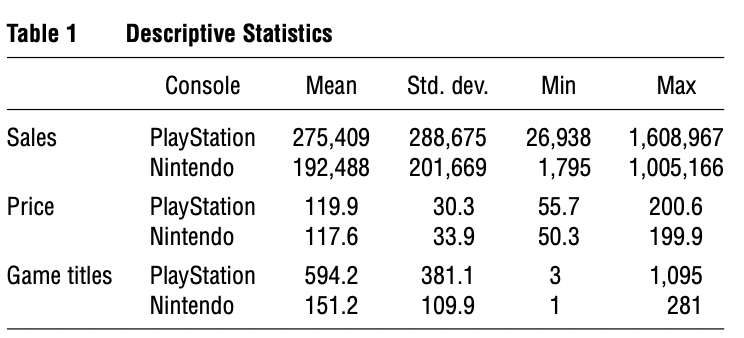
\includegraphics[scale=0.5]{resources/dube-table1}\\
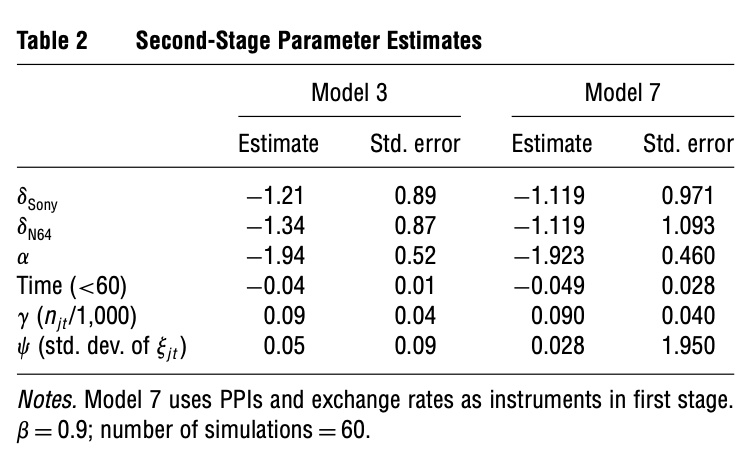
\includegraphics[scale=0.5]{resources/dube-table2}
\end{center}
\end{frame}

\begin{frame}{Counterfactual}
Suppose we got rid of network effects, how much lower would the concentration of the market be?
\end{frame}

\begin{frame}{Results}
\begin{center}
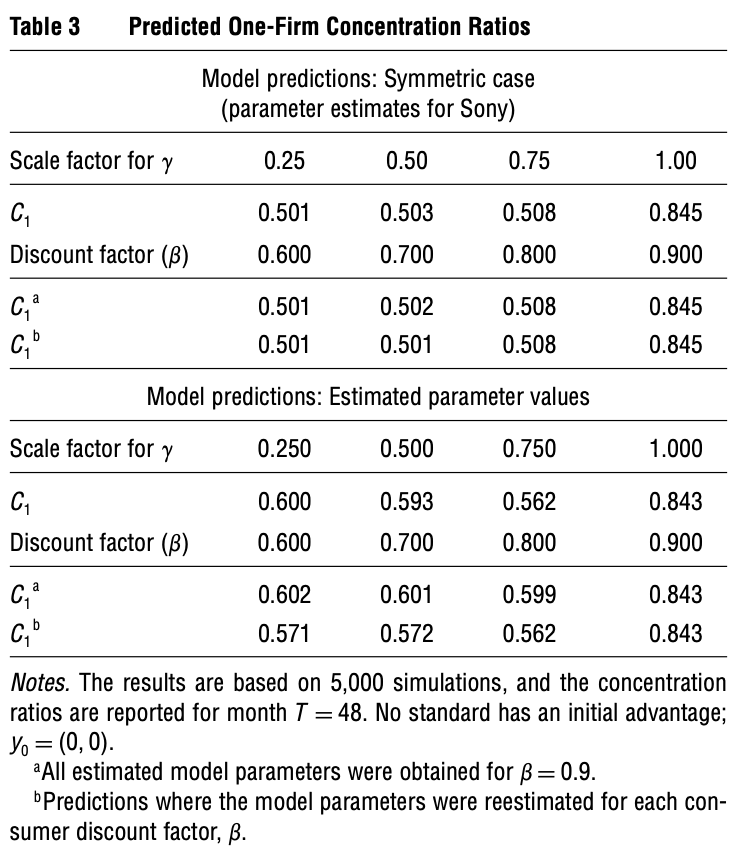
\includegraphics[scale=0.65]{resources/dube-table3}
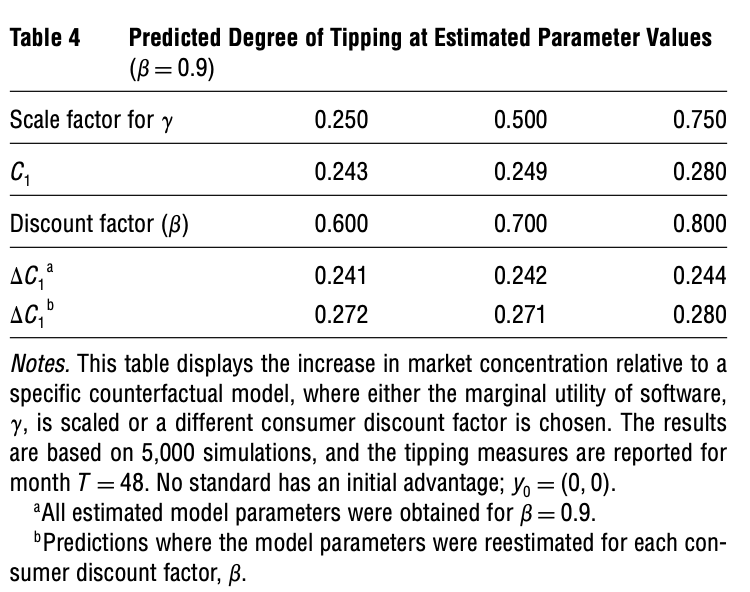
\includegraphics[scale=0.65]{resources/dube-table4}\\
\end{center}
\end{frame}

\begin{frame}{Results}
\begin{center}
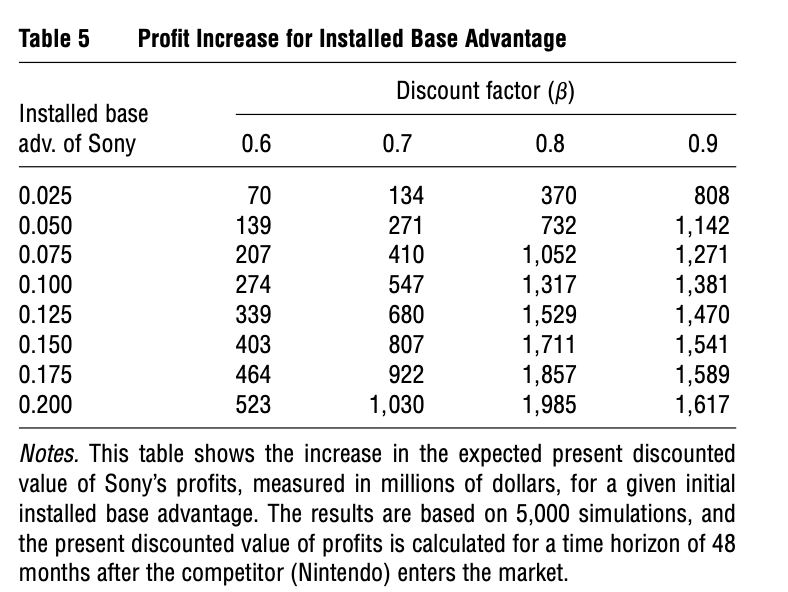
\includegraphics[scale=0.75]{resources/dube-table5}
\end{center}
\end{frame}


\end{document}













































